\section{approach}
\subsection{Approach Overview}
Our approach takes the coverage data and reported issues as input and outputs the non-covered branches with the associated issues. Figure 1 shows the high level design of Covana. Covana consists of three major components: observer component, pre-processing component and analysis component.The observer component is implemented as several Pex extensions and is attached to Pex for observing different events and collecting data. It collects the coverage data and reported issues and passed them to the pre-processing component. The pre-processing component remove the useless data and dump the data into binary files. The analysis component consumes the pre-processed data in files, carrys out the analysis on the data and outputs the relevant data for non-covered issues.
\subsection{Observer Component}
The observer component is implemented as three Pex extensions: (1) Branch coverage observer. (2) Field access observer. (3) Issues observer.
\subsubsection{Branch coverage observer}
The branch coverage observer is attached to Pex for collecting the branch coverage data. After all the generated tests are executed, it will enumerate the methods of the class under test, checks the coverage information of each branch inside a method and find out the non-covered branches. As Pex operates on the level of MSIL (MicroSoft Intermediate Language)\cite{HalleuxT08}, the observer also collects the IL offset of each non-covered branches for further analysis.
\subsubsection{Field access observer}
During the execution with the initial simple input, Pex collects the symbolic constraints along the path explored and flips one of the constraints to obtain a new path for the future executions. The field access observer is pluged into Pex for observing the events raised when Pex could not negate a constraint to obtain a new path. It will collect the information about the branch and the involved fields. 
\subsubsection{Issues observer}
The issue observer collects different kinds of issues reported by Pex, such as object creation issues, uninstrumented method issues and testability issues.
\subsection{Pre-processing Component}
The pre-processing component pre-processes the different kinds of data collected by the observer component, filters out the useless data based on some heuristics and save the data into binary files.  
\subsubsection{Filter out useless branch coverage data}
A test suite satisfying all branch coverage criteria always satisfies all statement coverage criteria, but not vice versa. Thus, when we get the data of all the non-covered branches, not all of them are useful for user since we focus on helping user to achieve higher block or statement coverage. 
\begin{figure}
\begin{CodeOut}
\begin{alltt}
    if (x != null) \{ 	
  	   Console.WriteLine("type: " + x.GetType());
    \}
    IEnumerator xe = x.GetEnumerator();
\end{alltt}
\end{CodeOut}
\Caption{Non-covered branch with full block coverage when x is not null}
\label{fig:useless1}
\end{figure}

\begin{figure}
\begin{CodeOut}
\begin{alltt}
    if (x == null || y == null) \{ 	
  	   return true;
    \}
    return false;
\end{alltt}
\end{CodeOut}
\Caption{Non-covered branch with full block coverage when x is not null but y could be null}
\label{fig:useless2}
\end{figure}
Figure \ref{fig:useless1} shows an example of code under test which achieves full block coverage but not branch coverage. In the example, x is the class under test and is assumed to be not null. In this case, if x is not null, the test case achieves full block coverage but not full branch coverage since the false branch of ``x != null'' is not covered. However, even we make this branch covered, it won't increase the statement or block coverage as it is already covered. Hence, we could simply filter out such non-covered branches. To find out such kind of non-covered branches, we need to check the coverage of their target statements. If their target statements are already covered, then these non-covered branches are considered useless and could be safely filtered out. (later we may deal with the situation of multi clause, like ``if(x!=null || y != null)'' showed in Figure \ref{fig:useless2})
\subsubsection{Filter out field access information of covered branches}
The field access information is collected when Pex fails to negate a constraint on a branch. However, Pex does not just stop exploration due to its failing to flip a constraint. It will try to flip other constraints and this may result in a path which covers the branch. Hence, when the field access information going through the pre-processing component, we will filter out the filed access information of the covered branches.
\subsection{Analysis Component}
The analysis component reads the pre-processed data from binary files and carrys out the analysis on it. It filters out the unrelevant issues, classifies issues into the defined categories and reports the non-covered issues with the related issues. 
\subsubsection{Object Creation Issue}
To find out whether an object creation issue is related to a non-covered branch or not, we need to examine the information about the field access information for the non-covered branches and object creation issues reported. As the pre-processed component has filtered out the field access information of the covered branches, the remaining field access information could be used directly for the analysis. Our approach thus picks up object creation issues one by one and check whether the type of each reported object is the same as the type of some field involved in non-covered branches. If yes, we consider the this object creation issue is relevant to the non-covered branch and assign it to the branch, which will be reported together later. Otherwise, we just simply ignore the issue.
\subsubsection{External Library Dependency Issue}
We use the latest feature of Pex to track the return value of each uninstrumented method. If it is involved in some branch where Pex fails to cover, then we will report it. (This part could be implemented using Nikolai's newly released feature of Pex)
\subsubsection{Environment Dependency Issue}
We could check whether the non-covered branch involves some static method call(File.Exists) or method calls of some environment dependency objects (socket for network connection, ADO.NET for database and other common .NET library for environment interaction). We could define a set of these library names and if we find them in some non-covered branch, we could simply consider this is the environment dependency issue.
\subsubsection{Loop Issue}
This may not be so easy. But the current clue I find is that inside a long run loop, the problem information collected when Pex tries to solve a problem will have many similar constraints. The code I use for testing is showed in Figure \ref{fig:loop}. Figure \ref{fig:problem} shows the problem log I got. They all occurs at the same line and the reason why they always choose to flip the n.length is because of the fitness strategy. To know whether there is a loop issue or not, we could check whether Pex report path boundary or not.

\begin{figure}
\begin{CodeOut}
\begin{alltt}
public static void LargeLoop(int[] number)
\{
     for (int i = 0; i < 5000; i++)
     \{
          for (int j = 0; j < number.Length - i - 1; j++)
          \{
              if (number[j] > number[j + 1])
              \{
                  int temp = number[j];
                  number[j] = number[j + 1];
                  number[j + 1] = temp;
              \}
          \}
     \}
     if (number.Length > 5000)
     \{
          throw new Exception("bug");
     \}
\}
\end{alltt}
\end{CodeOut}
\Caption{Long run loop for test}
\label{fig:loop}
\end{figure}

        
\begin{figure}
\begin{CodeOut}
\begin{alltt}
flipped location:  line: 12
return 59 < n.Length;

flipped location:  line: 12
return 60 < n.Length;

flipped location:   line: 12
return 61 < n.Length;

flipped location:  line: 12
return 62 < n.Length;

flipped location:  line: 12
return 63 < n.Length;

flipped location:  line: 12
return 64 < n.Length;
\end{alltt}
\end{CodeOut}
\Caption{Part of the problem log of Pex for long run loop}
\label{fig:problem}
\end{figure}


%\begin{figure}%
%\includegraphics[scale=0.4, trim=0 120mm 100mm 0mm]{code1.eps}%l b r t
%\caption{}%
%\label{sample}5t
%\end{figure}

